\documentclass[compress]{beamer}
\usetheme{Warsaw}
\usecolortheme{wolverine}
\usefonttheme[onlylarge]{structurebold}
\setbeamerfont*{frametitle}{size=\normalsize,series=\bfseries}
\setbeamertemplate{navigation symbols}{}
\setbeamertemplate{footline}
{%
\begin{beamercolorbox}[wd=0.5\textwidth,ht=3ex,dp=1.5ex,leftskip=.5em,rightskip=.5em]{author
in head/foot}%
\usebeamerfont{author in head/foot}%
\hfill\insertshortauthor%
\end{beamercolorbox}%
\vspace*{-4.5ex}\hspace*{0.5\textwidth}%
\begin{beamercolorbox}[wd=0.5\textwidth,ht=3ex,dp=1.5ex,left,leftskip=.5em]{title
in head/foot}%
\usebeamerfont{title in head/foot}%
\insertshorttitle\hfill\insertframenumber/\inserttotalframenumber%
\end{beamercolorbox}%
}
\beamertemplatesolidbackgroundcolor{black!5}
\beamertemplatetransparentcovered

\usepackage[utf8]{inputenc}
\title{Das Freie Betriebsystem Linux}
\author{Frank Lanitz \\ \tiny{frank@frank.uvena.de}}
\date{\today}
\begin{document}
\frame{\titlepage}
\begin{frame}
	\tableofcontents{}
\end{frame}
\begin{frame}
	\frametitle{Vorstellungsrunde}
	\begin{block}{Über mich}
		\begin{itemize}
			\item Bis letzte Woche Systembetreuer an der Universität Jena 
				\begin{itemize}
					\item Linux
					\item PostgreSQL
					\item ...
				\end{itemize}
			\item Jetzt: Administrator bei der Max-Planck-Gesellschaft
			\item Im Vorstand des Hackspace Jena e.V.
			\item Aktiv im Umfeld der FLOSS (u.a. seit 7 Jahren bei Geany)
			\begin{itemize}
				\item Übersetzungen
				\item Maintainer verschiedener Plugins
				\item Mailingliste, IRC, \dots
			\end{itemize}
		\end{itemize}
	\end{block}
\end{frame}
\begin{frame}
	\frametitle{Das Publikum}
	\center{\Huge{Wer seit Ihr so?}}
\end{frame}
\begin{frame}
	\tableofcontents{}
\end{frame}
\section{Freie Software}
\subsection{Urheberrecht, Copyright \dots}
\begin{frame}
	\frametitle{Urheberrecht und Copyright}
	\textbf{Achtung: Ich bin kein Anwalt \dots}
	\pause
	\begin{block}{Allgemein}
		\begin{itemize}
			\item Urheberrechte/Copyright wohnt allem Geschaffenen inne
			\item Allgemein gilt: Recht auf Festlegung, was mit einem Werk 
				passiert
			\item Auslegungsunterschiede je nach Rechtsraum
		\end{itemize}
	\end{block}
	\pause
	\begin{block}{Deutschland}
		\begin{itemize}
			\item Urheberrecht kann nicht abgegeben werden
			\item Software wird sowohl Binär als auch in Quellcode geschützt; 
				Darüber hinaus analog zu Sprachwerken (§ 69a Abs 4 UrhG)
			\item Nutzer muss eine Lizenz zur Verwendung haben (z.B. EULA)
		\end{itemize}
	\end{block}
	\pause
	\textbf{Aber: Ich bin kein Anwalt \dots}
\end{frame}

\subsection{Freie Software}

\begin{frame}
	\frametitle{Freie Software}
	\begin{block}{}
		\begin{itemize}
			\item Unterscheidung zwischen Freeware und freier 
				Software (free software)
			\item “Free as in ‘freedom’, not as in ‘free beer’”
				(Richard Stallman)
			\item Verschiedene Definitionen und Lizenzen (BSD, MIT, 
				Apache, GPL, LGPL, AGPL, Beerware \dots{})
			\item Merkmale von Open Source
			\begin{enumerate}
				\item Quellcode liegt in lesbarer und verständlicher Form vor
				\item Quellcode darf beliebig oft kopiert, verbreitet und 
					genutzt werden
				\item Quellcode darf verändert und in der veränderten Form 
					weitergegeben werden
			\end{enumerate}
		\end{itemize}
	\end{block}
\end{frame}

\begin{frame}
	\frametitle{Finanzierung}
	\begin{block}{Prämisse}
		\begin{itemize}
			\item Das Problem steht vor der Lösung
		\end{itemize}
	\end{block}
	\pause
	\begin{block}{Finanzierung von FLOSS}
		\begin{itemize}
			\item Auftragsarbeiten: "Ich benötige ein Programm, um XYZ 
				zu machen"
			\item Kommerzieller Support
			\item Spenden
			\item Merchandising 
		\end{itemize}
	\end{block}
	\pause
	$\rightarrow$ Datenkanal 002 (\url{http://yaturl.net/cdaa})
\end{frame}

\section{Betriebsystem}

\begin{frame}
	\frametitle{Betriebssystem}
	\begin{center}
	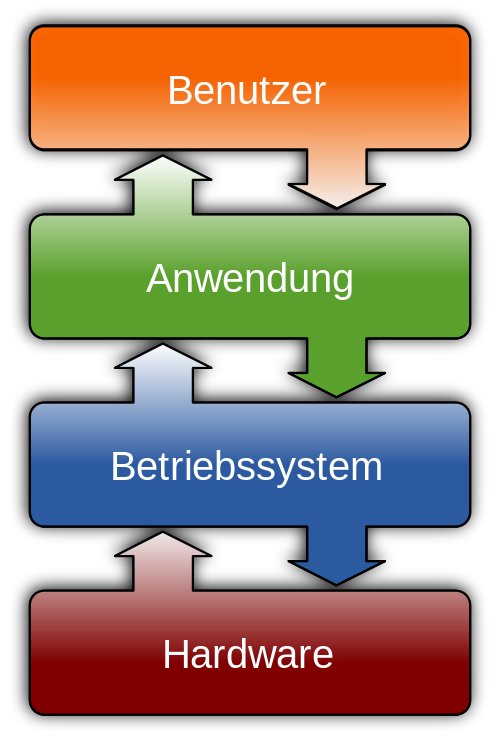
\includegraphics[scale=0.25]{media/500px-Operating_system_placement-de.png}
	\end{center}
	\raggedleft{\tiny aus der Wikipedia}
\end{frame}

\begin{frame}
	\begin{block}{}
		\begin{itemize}
			\item Viele verschiedene Systeme 
			\item Anwendungsspezifisch optimiert
				\begin{itemize}
					\item Echtzeit
					\item Minimalistisch
					\item General
					\item Desktop/Server
					\item Mobile Geräte 
				\end{itemize}
		\end{itemize}
	\end{block}
	\begin{block}{Beispiele}
		\begin{itemize}
			\item DOS - Disc Operating System
			\item Microsoft Windows
			\item Unixoide Systeme
				\begin{itemize}
					\item GNU/Linux
					\item *BSD: Open/Free/PC/Dragefly/Net
					\item AIX
					\item MacOS X
				\end{itemize}
		\end{itemize}
	\end{block}
\end{frame}

\begin{frame}
	\frametitle{Umfang \& Architektur}
	\begin{block}{Umfang des Betriebssystem}
		\begin{itemize}
			\item Aus einem Guß: MaxOS X, 
				Mcrosoft Windows XY\footnote{mit Abstrichen}, PC-BSD
			\item Minimalistisch: Klassische Unix-Systeme
			\item Nur das wichtigste: GNU/Hurd, Linux, Minix
		\end{itemize}
	\end{block}
	\pause{}
	\begin{block}{Architektur}
		\begin{itemize}
			\item \textbf{Monolitisch:} Alle Treiber und Funktionen sind 
				in einem Paket
			\item \textbf{Modular:} Treiber \& Funktionen kommen als 
				einzelne Module
		\end{itemize}
	\end{block}
\end{frame}

\section{Linux}

\begin{frame}
	\frametitle{Linux -- Nur der Kern}
	\begin{columns}[c]
		\column[c]{4cm}
			
\includegraphics[scale=0.5]{media/tux.png} \newline
			\huge Linux
		\column{6cm}
			\pause
			\begin{block}{}
				\begin{itemize}
					\item Linux (im All.) ist eine Sammlung von Programmen
					\item Linux (im Spez.) ist der Betriebssystemkern
					\item Wurde ursprünglich 1991 von Linus Torvalds 
						veröffentlicht
					\item Lizenz: GPL2
					\item Gemeinsam mit den um Richard Stallman entwickelten 
						GNU-Programmen $\rightarrow$ GNU/Linux
				\end{itemize}
			\end{block}
	\end{columns}
\end{frame}

\begin{frame}
	\frametitle{Bezugsquellen von Linux}
	\begin{block}{}
		\begin{itemize}
			\item Linux kommt in der Regel als Distribution
			\item Distribution:
				\begin{itemize}
					\item Vorauswahl von Programmen
					\item Grundkonfigurationen \& Abstimmung aufeinander
					\item Bestimmte Zielgruppe
					\item Meist: Fehlerkorrekturen, Dokumentation, Support
					\item Beispiele: Ubuntu, Debian, openSuSE/SuSE, RedHat, 
						Fedora, Slackware, Gentoo, Android, grml, Knoppix \dots{}
				\end{itemize}
			\item Aber: Komplett selbst zusammenstellen ist auch möglich 
				(z.B. \textbf{L}inux \textbf{F}rom \textbf{S}cratch 
				$\rightarrow$ LFS)
		\end{itemize}
	\end{block}
	\pause
	\begin{block}{Bezugsquellen}
		\begin{itemize}
			\item Download aus dem Internet
			\item Kauf eines Paketes, Linux Buchs oder einer Zeitschrift
			\item Vorinstalliert (z.B. Dell, Asus' eeePC)
		\end{itemize}
	\end{block}
\end{frame}

\begin{frame}
	\frametitle{Die Qual der Wahl - Auswahl wohin das Auge reicht}
	\begin{block}{}
		\begin{itemize}
			\item Für jedes Problem gibt es mindestens zwei Lösungen
			\pause{}
			\item Desktopumgebungen (bunte Fenster)
				\begin{itemize}
					\item Xfce
					\item KDF
					\item Gnome
					\item Mate
					\item Unity
					\item \dots{}
				\end{itemize}
			\pause
			\item Editoren
				\begin{itemize}
					\item Vim
					\item Emacs
					\item Geany
					\item mcedit
					\item nano
					\item \dots{}
				\end{itemize}
		\end{itemize}
	\end{block}
\end{frame}

\begin{frame}
	\frametitle{Vor- und Nachteile}
	\begin{block}{Pro}
		\begin{itemize}
			\item Große Auswahl
			\item Individual = Genaue Anpassung an Vorlieben
			\item Nicht zwingend abhängig von einer Software
		\end{itemize}
	\end{block}
	\pause{}
	\begin{block}{Contra}
		\begin{itemize}
			\item Große Auswahl
			\item Schwierig das passende Programm zu finden
			\item Abstimmung zwischen Programmen teils schwierig
		\end{itemize}
	\end{block}
	\pause{}
	\begin{block}{Lösung}
		\begin{itemize}
			\item Distributionen
			\item Nutzertreffen
		\end{itemize}
	\end{block}
\end{frame}

\begin{frame}
	\frametitle{Wo gibt es Hilfe}
	\begin{block}{}
		\begin{itemize}
			\item Handbücher, Fachbücher, Zeitschriften
			\item Internet: Newsgroups, Foren, Mailinglisten, IRC
			\item Kommerzeller Support
			\item Nette Leute, die gerne weiterhelfen (Linux User Group, 
				Freunde \& Bekannte)
		\end{itemize}
	\end{block}
\end{frame}

\begin{frame}
	\frametitle{Linux User Group Jena}
	\begin{block}{Werbung}
		Die LUG Jena trifft sich alle 2 Wochen zum Stammtisch.\\
		Nächster Termin: 4.10 19h im Hackspace Jena \\
		\url{http://lug-jena.de}
	\end{block}
\end{frame}

\begin{frame}
	\frametitle{Praxis}
	\center{}	\Huge{An das Gerät!}
\end{frame}

\end{document}
